

\subsection{Premier lancement}
	
		
	\paragraph{Création compte local\\}
	Au premier lancement de l'application il vous est demandé de créer un compte 
	local. Ce dernier est nécessaire pour pouvoir utiliser l'application. Il vous
	suffit de renseigner dans le champs prévu à cet effet, votre pseudonyme 1).
	\begin{center}
			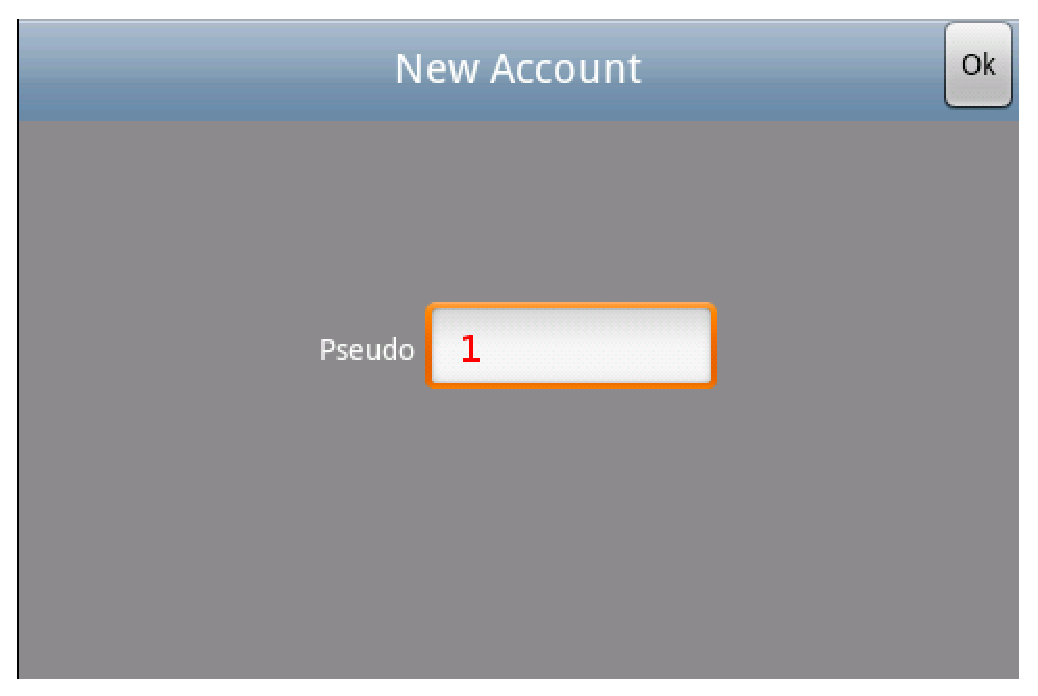
\includegraphics[scale=0.6]{Manuel/Img/2.eps}
	\end{center}

	
\subsection{Menu}	
	Le menu d'accueil vous permet d'accéder à la section des parties locales
	\textcolor{red}{\textbf{1}}, des parties multijoueurs
	\textcolor{red}{\textbf{2}}, l'éditeur de carte \textcolor{red}{\textbf{3}}
	pour créer vos propres cartes de jeu, le menu d'options
	\textcolor{red}{\textbf{4}}, l'accès aux comptes locaux
	\textcolor{red}{\textbf{5}}, la création d'un nouveau compte local
	\textcolor{red}{\textbf{6}} et enfin l'aide \textcolor{red}{\textbf{7}}.
	
	\begin{center}
			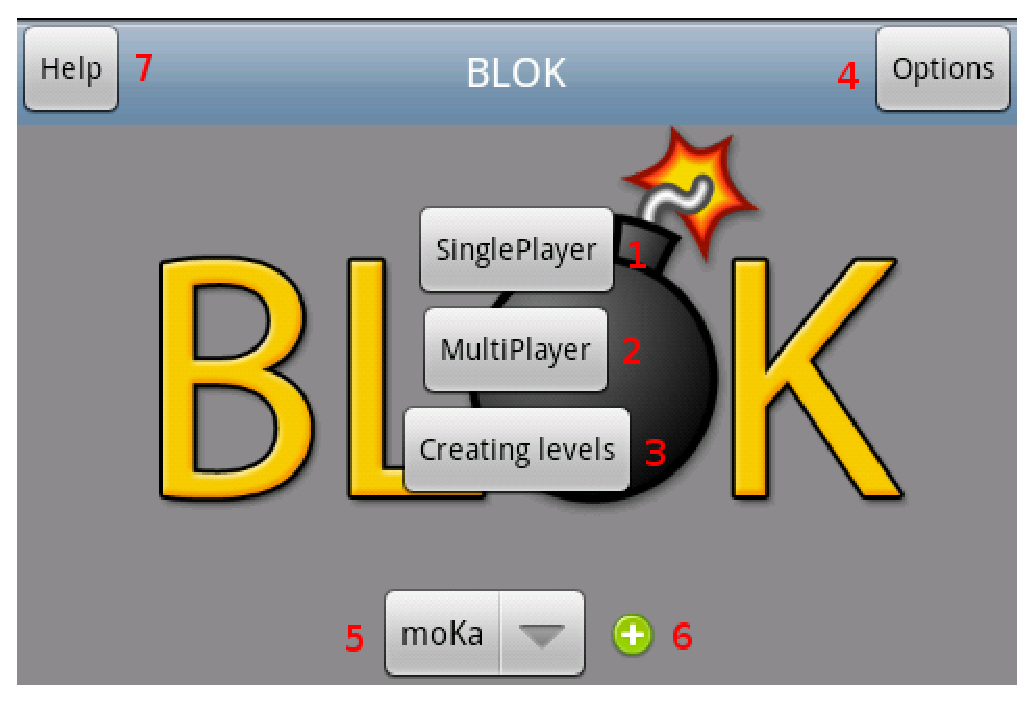
\includegraphics[scale=0.7]{Manuel/Img/3.eps}
	\end{center}
	
	
	
	\subsection{Jeu local \textcolor{red}{1}}
	\paragraph{Paramétrage\\}
	Voilà un moment crucial précédent votre lancement de jeu, sa configuration.
	Rien de bien compliqué en soit, vous choisissez le type de partie
	\textcolor{blue}{\textbf{2}}, la difficulté de vos adversaires(robots)
	\textcolor{blue}{\textbf{3}}, le nombre d'ennemis sur la carte
	\textcolor{blue}{\textbf{4}}, le temps de jeu \textcolor{blue}{\textbf{5}},
	et enfin grâce à un défilement de la galerie \textcolor{blue}{\textbf{1}}, la
	carte de jeu. Vous n'avez plus qu'à valider
	\textcolor{blue}{\textbf{7}} ou revenir au menu précédent
	\textcolor{blue}{\textbf{6}}.
	
	\begin{center}
		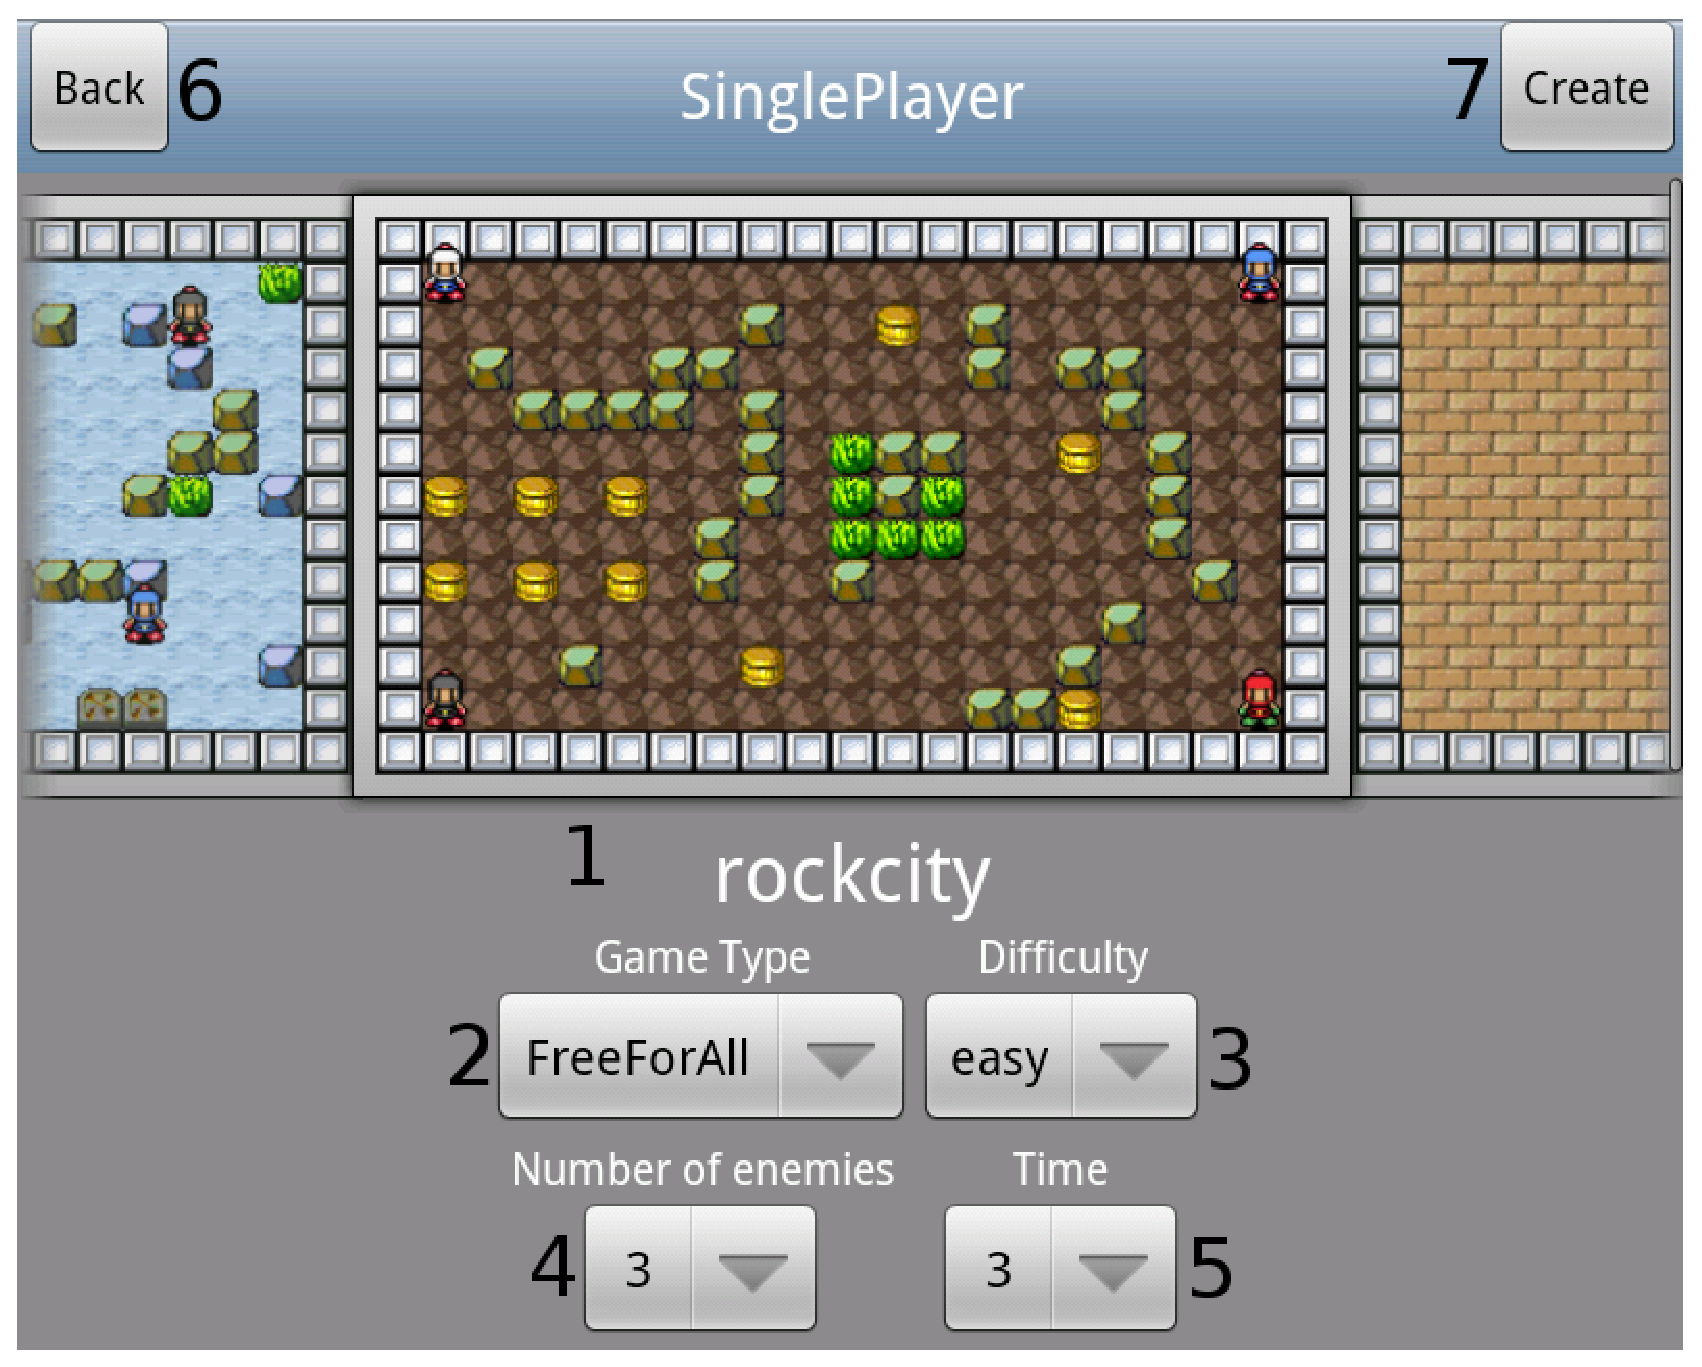
\includegraphics[scale=0.4]{Manuel/Img/15.eps}
	\end{center}
	
	\paragraph{Jeu\\}
	Après avoir choisi vos préférences pour votre partie, celle-ci se lance.
	Pour vous déplacer votre joueur, effleurez l'écran de jeu dans le sens et la
	direction où vous souhaiter aller \textcolor{blue}{\textbf{1}} .	
	Sur le panneau de droite en appuyant sur le
	bouton prévu \textcolor{blue}{\textbf{2}}, vous posez des bombes.
	Le panneau du haut résume les informations de la partie. Le temps de jeu
	\textcolor{blue}{\textbf{3}} restant, et vos différents bonus. Ces derniers
	correspondent à la portée de vos bombes \textcolor{blue}{\textbf{4}}, le
	nombres de bombes que vous pouvez poser
	simultanément \textcolor{blue}{\textbf{5}}, la vitesse de déplacement de votre
	joueur \textcolor{blue}{\textbf{6}}, et votre compteur de vies
	\textcolor{blue}{\textbf{7}}.
	
	\begin{center}
		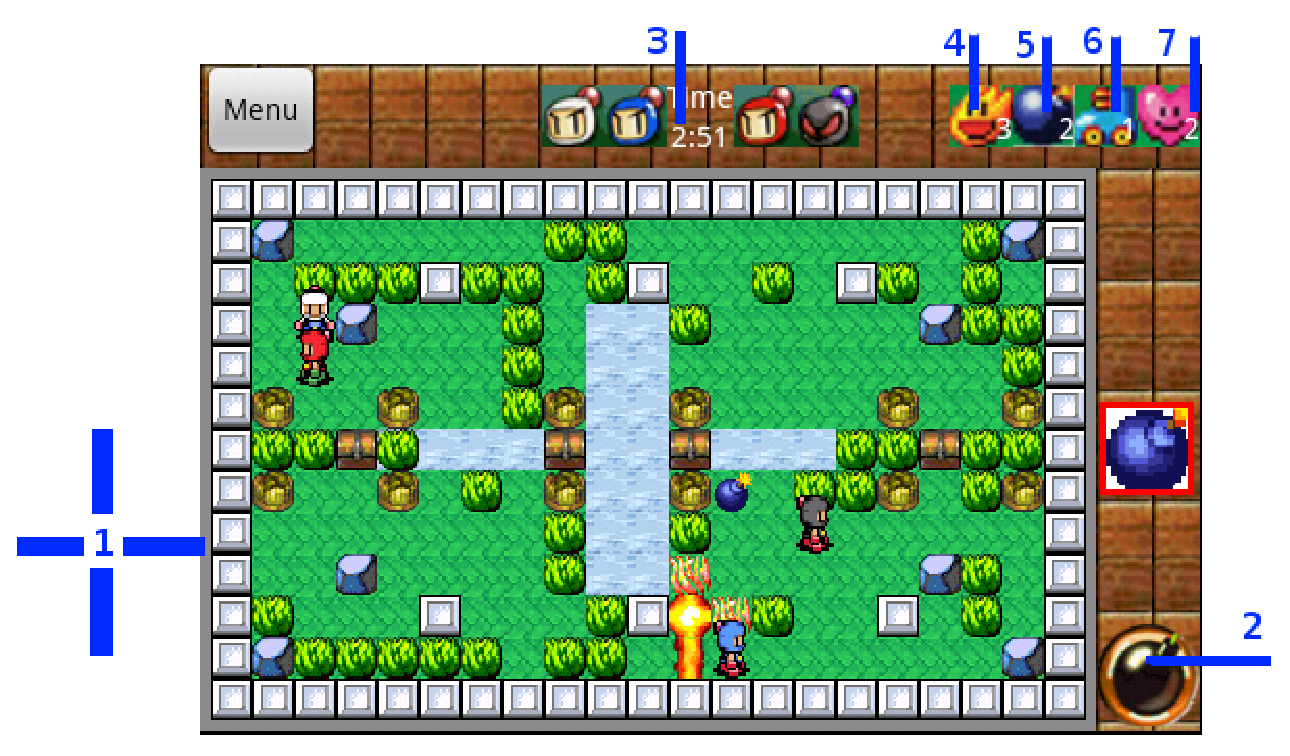
\includegraphics[scale=0.6]{Manuel/Img/21.eps}
	\end{center}
	
	\paragraph{Pause\\}
	Lors d'une partie vous pouvez la suspendre en appuyant sur le Menu
	\textcolor{orange}{\textbf{1}} en haut à gauche. Il vous est possible de
	reprendre la partie \textcolor{orange}{\textbf{2}}, accéder aux options de jeu
	\textcolor{orange}{\textbf{3}}, redémarrer la partie
	\textcolor{orange}{\textbf{4}}, ou tout simplement la quitter et revenir au
	menu \textcolor{orange}{\textbf{5}}. 
	
	\begin{center}
		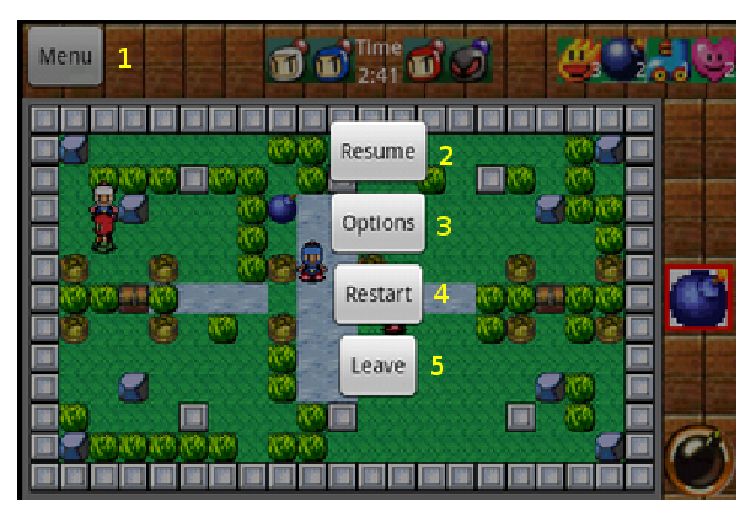
\includegraphics[scale=0.8]{Manuel/Img/20.eps}
	\end{center}


\subsection{Jeu multi \textcolor{red}{2}}

	\paragraph{Inscription}
	Cette étape est inévitable afin d'accéder au mode multijoueur. Vous devez
	renseigner userName \textcolor{blue}{\textbf{1}}, mot de passe
	\textcolor{blue}{\textbf{2}}, et confirmer ce dernier
	\textcolor{blue}{\textbf{3}}. Vous pouvez choisir une connexion automatique
	\textcolor{blue}{\textbf{4}} ou simplement ne pas ressaisir votre mot de passe
	aux connexions suivantes \textcolor{blue}{\textbf{5}}. Dès que ces champs sont
	remplis, validez via la connexion au serveur \textcolor{blue}{\textbf{6}}. Le
	userName est unique, s'il est déjà pris le serveur vous renverra une erreur,
	sinon vous accéderez à l'Accueil du mode multijoueur.
	
	
	\begin{center}
		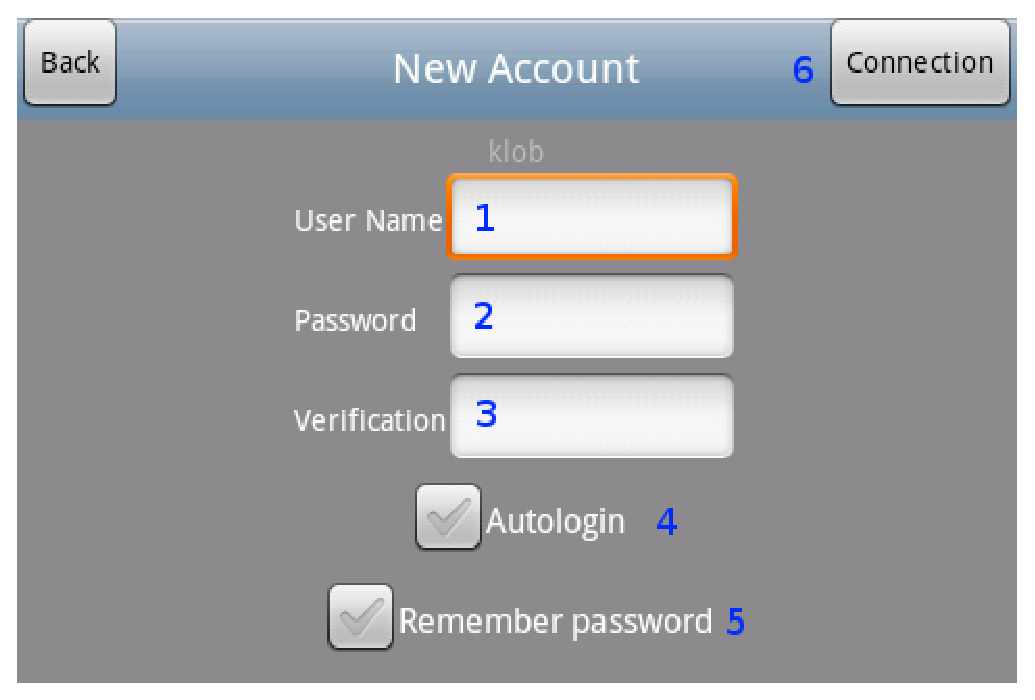
\includegraphics[scale=0.7]{Manuel/Img/18.eps}
	\end{center}
	
	\paragraph{Connexion}
		Une fois seulement l'étape précédente accomplie, vous pouvez passer par le
		menu de connexion. Dans ce dernier il faut donner le couple
		userName \textcolor{blue}{\textbf{1}}/mot de passe
		\textcolor{blue}{\textbf{2}}. Vous pouvez aussi choisir, dans le cas d'une
		identification correcte, la mémorisation de votre compte
		\textcolor{blue}{\textbf{3}} c'est à dire un accès direct sans passer par le
		menu de connexion, ou la mémorisation unique de votre mot de passe
		\textcolor{blue}{\textbf{4}}. Enfin il est toujours possible de créer un
		nouveau compte multijoueur \textcolor{blue}{\textbf{5}}. Là encore une
		vérification sur le serveur est faite lorsque vous choisissez la connexion
		\textcolor{blue}{\textbf{6}}.
		
		\begin{center}
			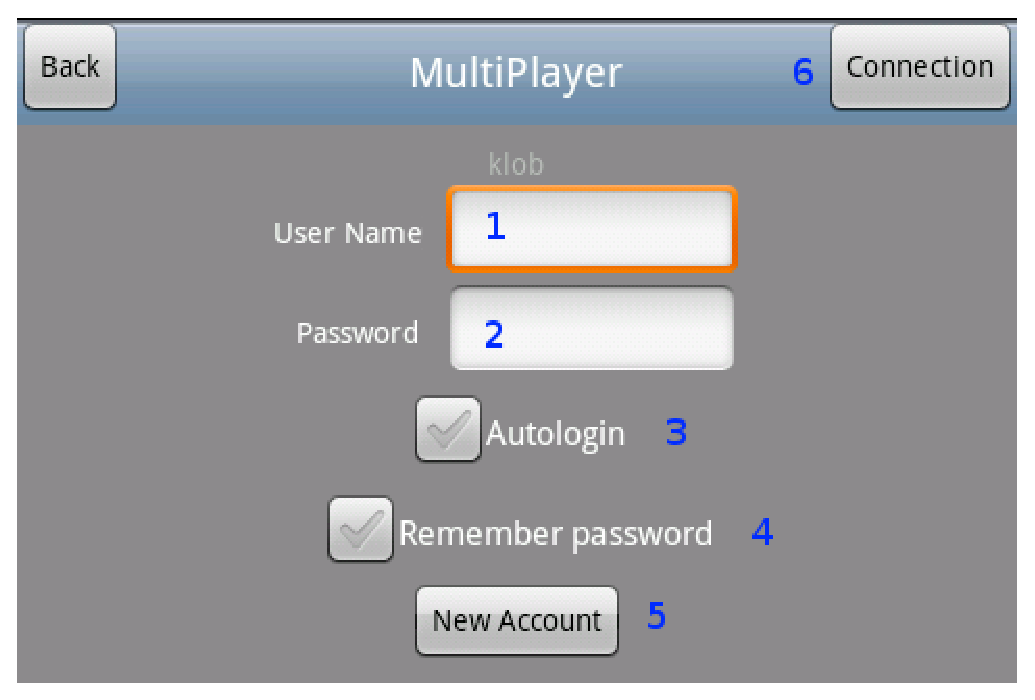
\includegraphics[scale=0.7]{Manuel/Img/17.eps}
		\end{center}
	
	\paragraph{Accueil}
	L'accueil du mode multijoueur est composé d'un champ éditable, permettant le
	tri des parties en lignes \textcolor{blue}{\textbf{1}}, le rafraîchissement des
	parties \textcolor{blue}{\textbf{2}}, une liste déroulante cliquable de celles
	en cour \textcolor{blue}{\textbf{3}}, et enfin un accès au menu de création
	d'une nouvelle \textcolor{blue}{\textbf{4}}.
	
		
	\begin{center}
		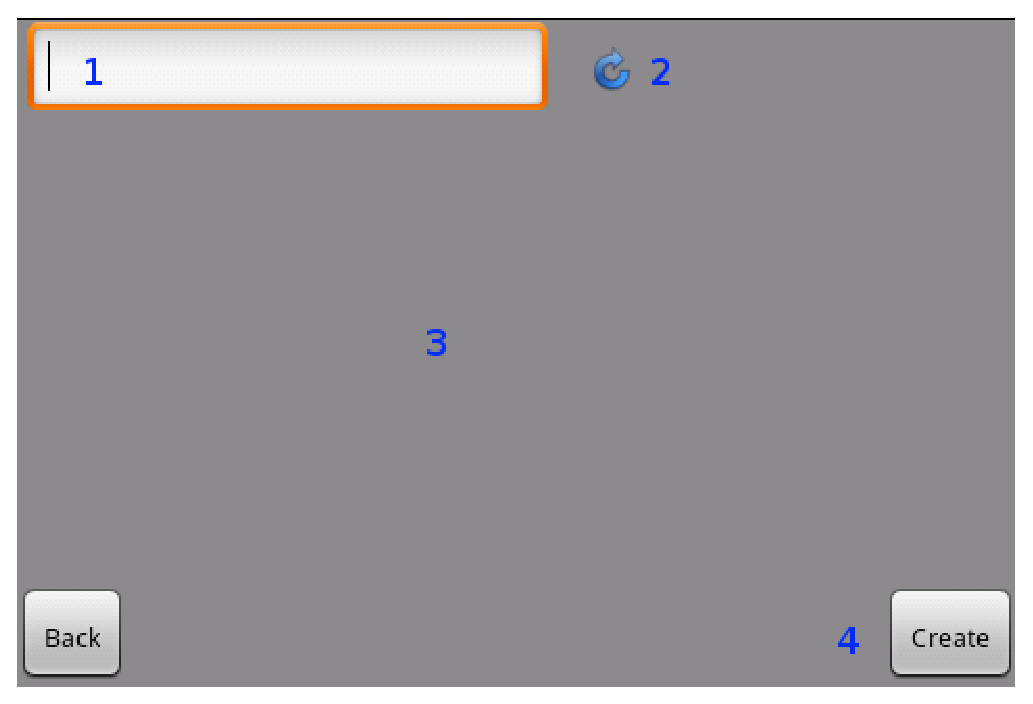
\includegraphics[scale=0.6]{Manuel/Img/19.eps}
	\end{center}
	
	\paragraph{Créer partie}
	La création multijoueur et semblable à celle en locale.
	Vous choisissez le type de partie
	\textcolor{blue}{\textbf{2}}, le nombre
	d'ennemis sur la carte \textcolor{blue}{\textbf{3}}, et le temps de jeu
	\textcolor{blue}{\textbf{4}}, et enfin grâce à un défilement de la galerie
	\textcolor{blue}{\textbf{1}}, la carte de jeu. Vous pourrez revenir au menu
	précédent \textcolor{blue}{\textbf{5}} ou vous validerez
	\textcolor{blue}{\textbf{6}} pour créer la partie.
	
	\begin{center}
		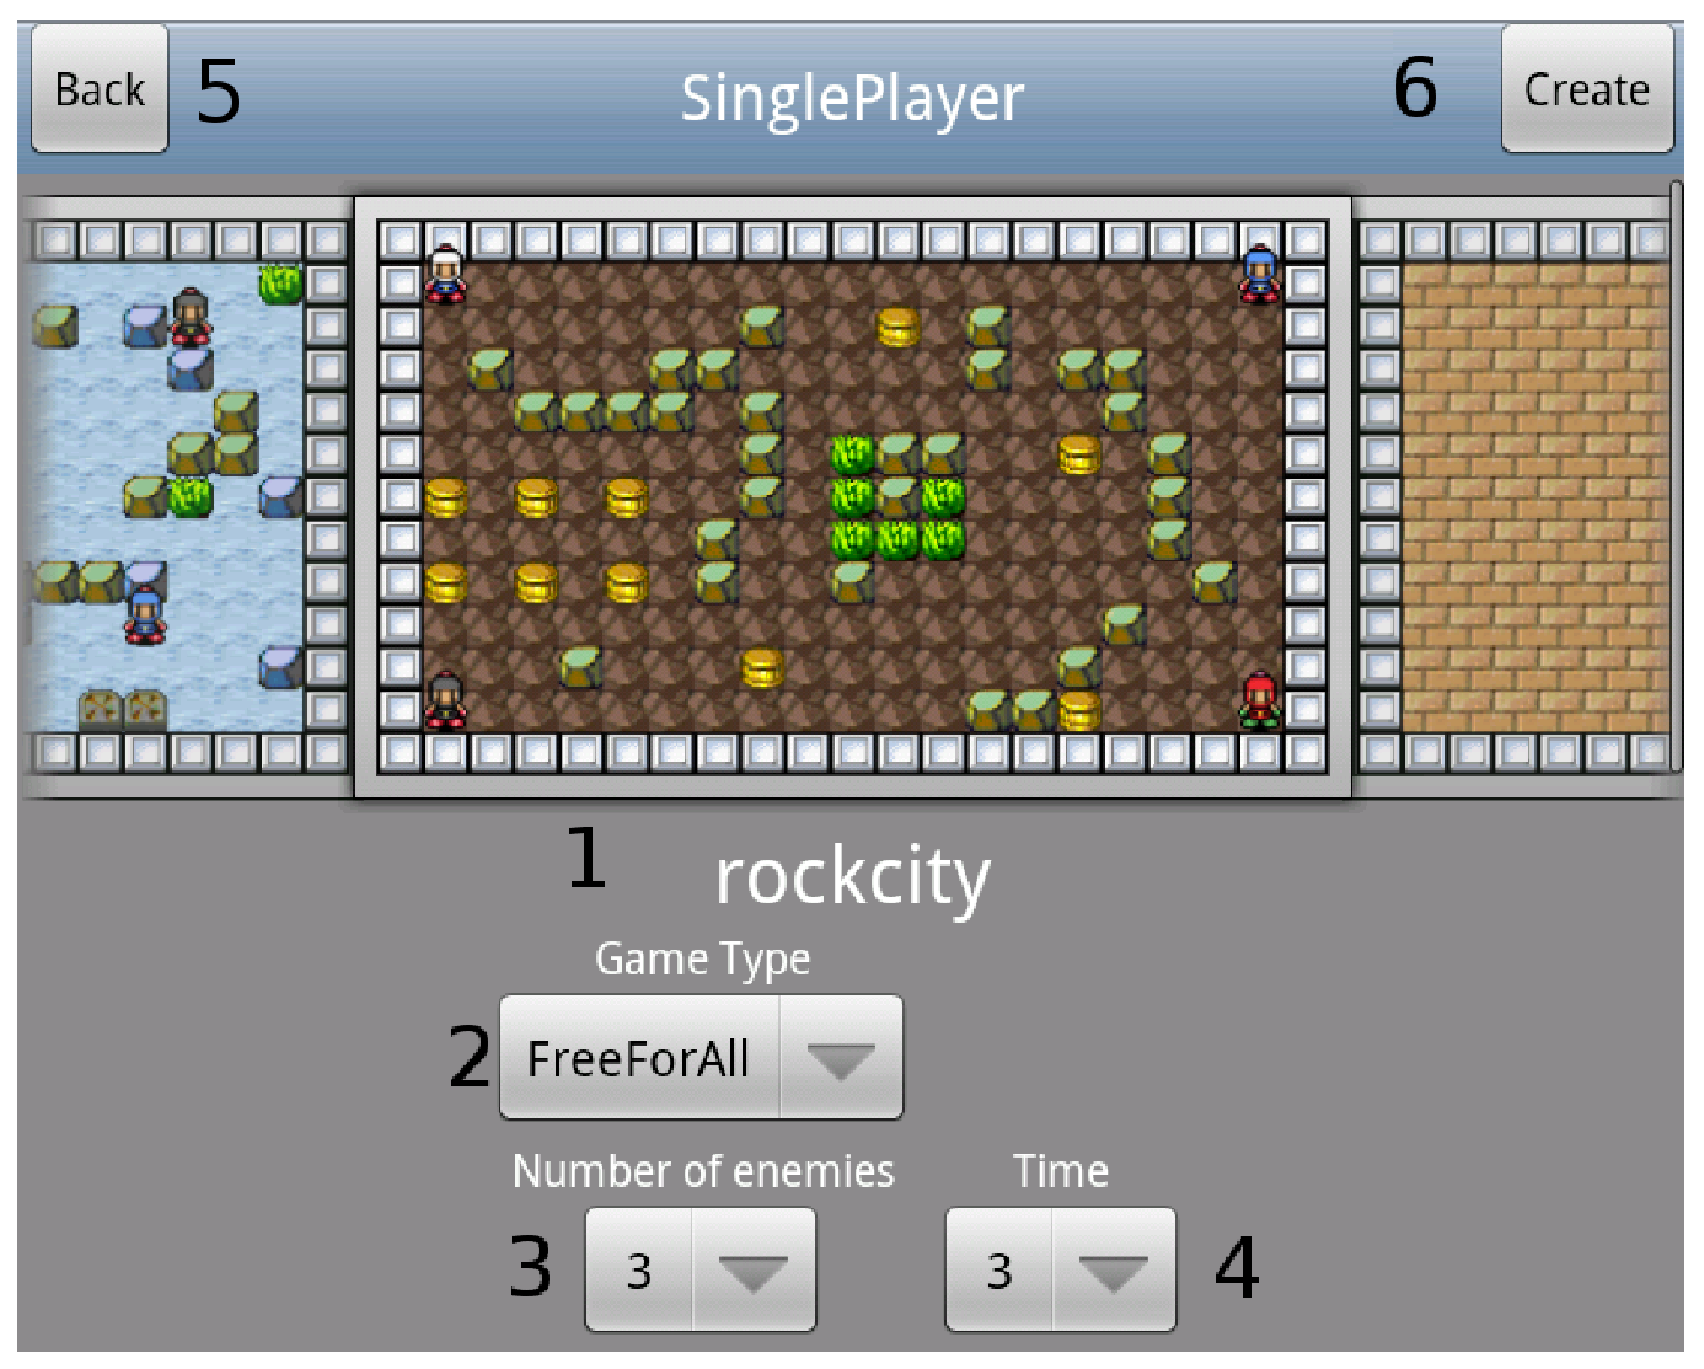
\includegraphics[scale=0.4]{Manuel/Img/16.eps}
	\end{center}
	
	
\subsection{Editeur de map \textcolor{red}{3} }
	
	\paragraph{Création de map\\}
	Comme dans tout jeux d'arcade qui se respecte, vous avez la possibilité de
	créer vos niveaux via un éditeur. Vous n'avez qu'à donner le nom de la carte
	\textcolor{blue}{\textbf{1}} que vous souhaitez créer puis valider
	\textcolor{blue}{\textbf{2}}. La encore les doublons ne sont pas possibles.
	
	\begin{center}
			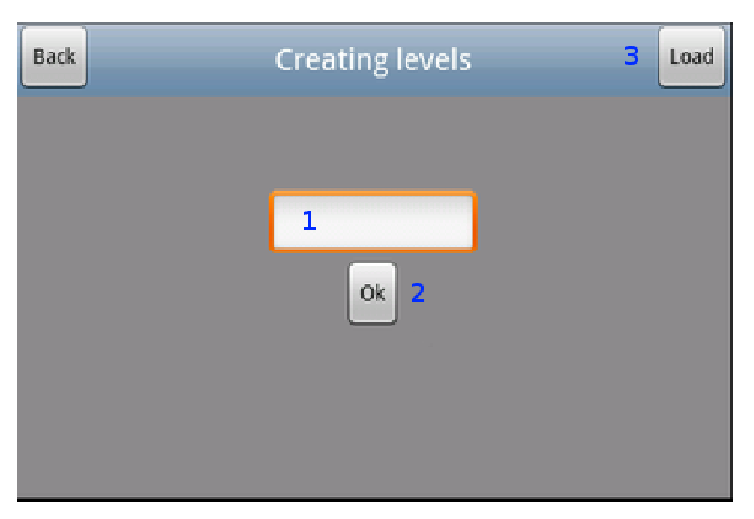
\includegraphics[scale=0.9]{Manuel/Img/10.eps}
	\end{center}

	
	\paragraph{Edition de map\\}
	Une carte vierge s'offre à vous \textcolor{blue}{\textbf{1}}. Le choix des
	structures(destructibles ou non) \textcolor{blue}{\textbf{2}}, de la texture du
	sol \textcolor{blue}{\textbf{2'}} mais aussi le positionnement des joueurs
	\textcolor{blue}{\textbf{3}} vous est alors mis à disposition. Pour passer des
	structures aux textures du sol, utilisez l'interrupteur situé en haut à droite
	de l'écran \textcolor{blue}{\textbf{4}}. Vous pourrez ensuite choisir l'image
	que vous souhaitez dessiner. Remarquez qu'en slidant de haut en bas, les images
	défilent ainsi, et inversement. Pointez sur la case que vous souhaitez dessiner
	avec la structure ou la texture pour dessiner une case. Il est aussi possible de rester appuyer sur l'écran tout en
	glissant, l'image choisit est alors appliquée sur toutes les cases survolées.
	
	
	\begin{center}
		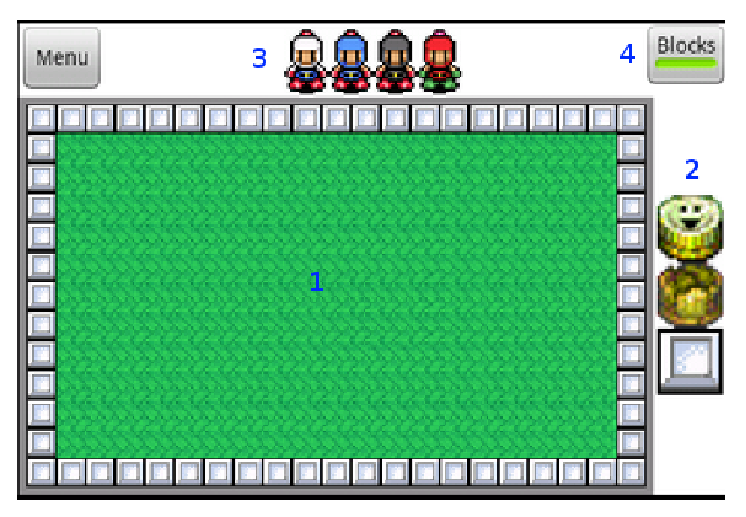
\includegraphics[scale=0.9]{Manuel/Img/11.eps}
	\end{center}
	
	\paragraph{Enregistrement map\\}
	Une fois votre carte achevée ou non, vous pouvez accéder au menu d'option
	via le bouton Menu \textcolor{orange}{\textbf{1}} . Ce dernier vous propose
	alors de retourner sur l'éditeur \textcolor{orange}{\textbf{2}}, d'enregistrer votre
	carte et quitter \textcolor{orange}{\textbf{3}}, de remettre à zéro votre carte
	\textcolor{orange}{\textbf{4}}, et enfin quitter sans enregistrer
	\textcolor{orange}{\textbf{5}}. 
	
	\begin{center}
		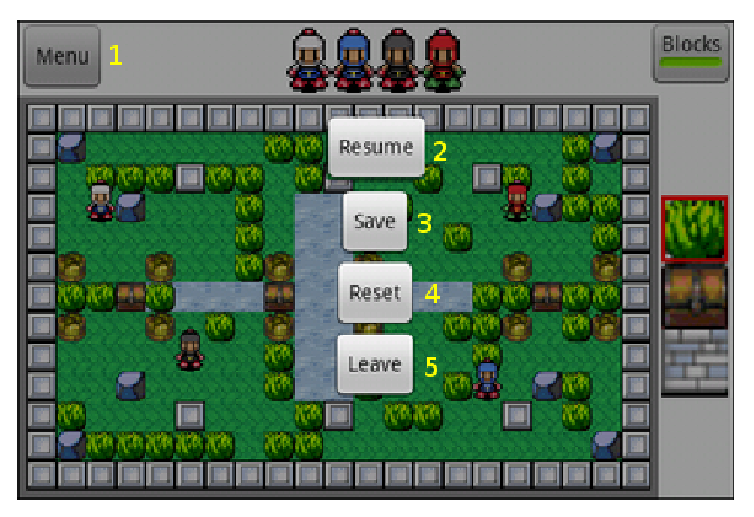
\includegraphics[scale=0.9]{Manuel/Img/13.eps}
	\end{center}
	
	\paragraph{Charger map\\}
	Après avoir enregistré une carte que vous ou un autre compte local aurait crée,
	il vous est possible de l'éditer et de l'enregistrer et ce en la choisissant
	\textcolor{blue}{\textbf{1}} parmi toutes les cartes crées et de valider
	\textcolor{blue}{\textbf{2}}. 
	
	\begin{center}
		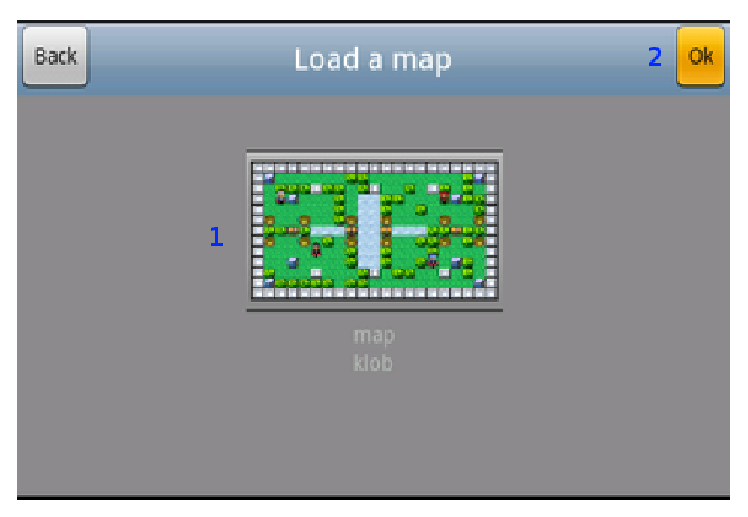
\includegraphics[scale=0.9]{Manuel/Img/14.eps}
	\end{center}
	

\subsection{Options \textcolor{red}{4}}
	Le menu d'option est à votre disposition pour régler vos paramètre systèmes
	mais aussi le profils d'utilisateur local et multiplayer.
	
	\paragraph{Réglage sytème\\}
	Ce type de réglage a été conçu pour ajuster le son
	\textcolor{blue}{\textbf{1}} à votre convenance mais aussi choisir la langue
	\textcolor{blue}{\textbf{2}} utilisée dans votre jeu. Sont à votre disposition
	le français mais aussi l'anglais.
	
	\begin{center}
		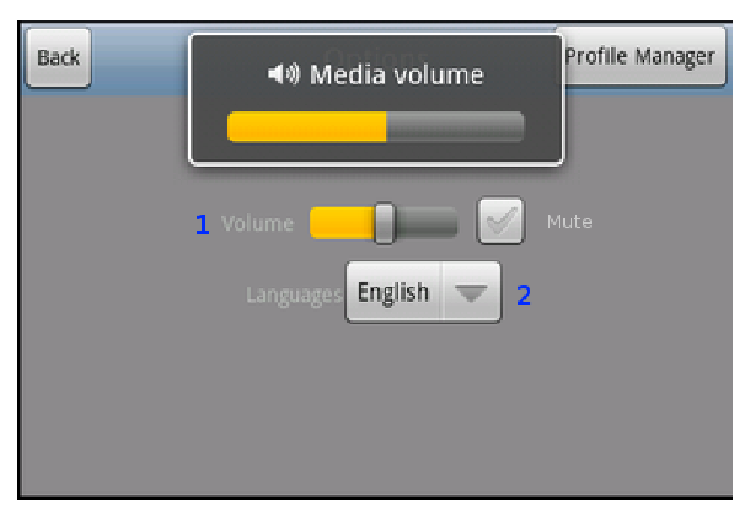
\includegraphics[scale=0.8]{Manuel/Img/4.eps}
	\end{center}
	
	\subsubsection{Gestionnaire profil}
		Dans ce menu vous avez accès à l'édition de vos profils locaux et
		multijoueurs. Une fois vos modifications accomplies n'oubliez pas de les
		valider en cliquant sur le bouton Ok situé en haut à droite de votre fenêtre.
		\paragraph{Local\\}
		Il vous est ici possible de changer le pseudonyme \textcolor{blue}{\textbf{1}}
		de votre compte local en cour, mais aussi de choisir la couleur de votre
		personnage \textcolor{blue}{\textbf{2}}, toujours pour les parties locales.
		\begin{center}
				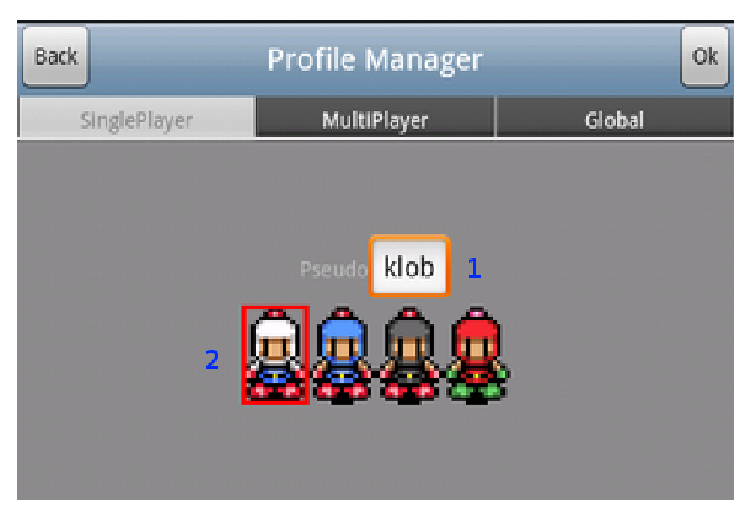
\includegraphics[scale=0.8]{Manuel/Img/5.eps}
			\end{center}
		
		\paragraph{Multijoueur\\}
		Une fois un compte multijoueur crée sur le serveur, cet onglet vous donnera la
		possiblité d'éditer \textcolor{blue}{\textbf{1}} userName et password mais
		aussi de changer de compte multijoueur \textcolor{blue}{\textbf{2}}. Les
		paramètres d'accès comme la connexion automatique
		\textcolor{blue}{\textbf{3}} ou la sauvegarde du mot de passe
		\textcolor{blue}{\textbf{4}} sont ici configurables dès lors que le couple
		userName/password sera renseigné et valide.
		
		\begin{center}
				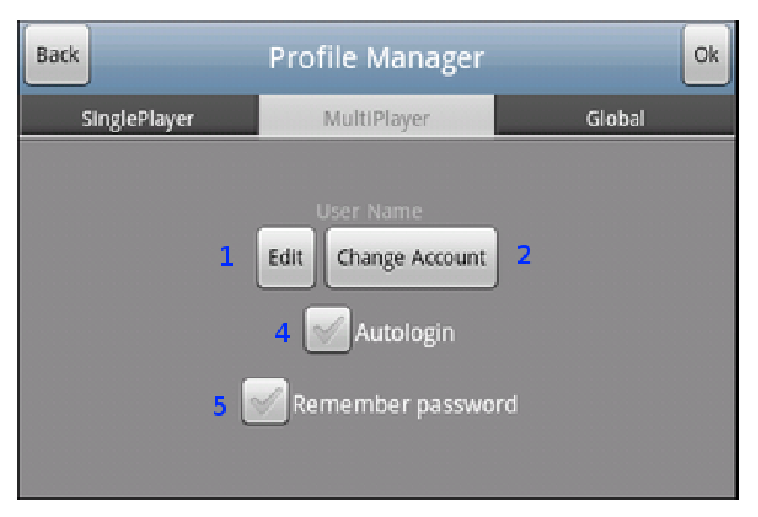
\includegraphics[scale=0.8]{Manuel/Img/6.eps}
		\end{center}
		
		\newpage{}	
		\paragraph{Général\\}
		Grâce au menu déroulant \textcolor{blue}{\textbf{1}}, vous pouvez fixer le
		côté de l'écran où est positionné le menu de jeu, c'est à dire celui contenant
		le bouton de posage de bombes pendant une partie, suivant si l'on est gaucher ou droitier. 
		
		\begin{center}
				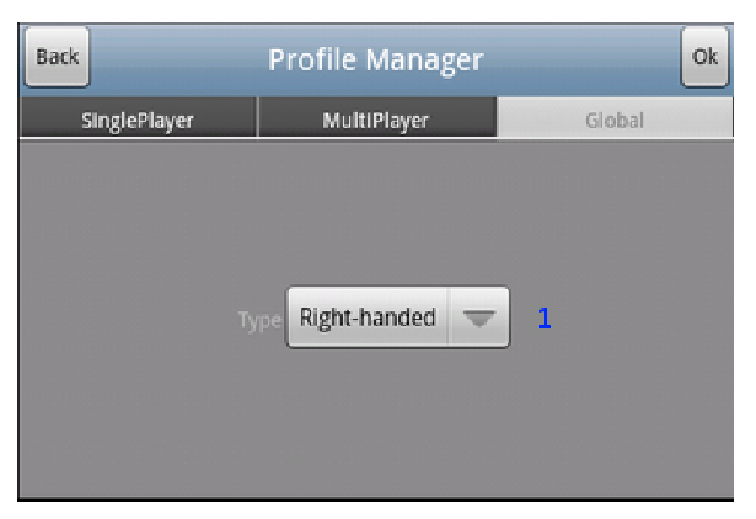
\includegraphics[scale=0.8]{Manuel/Img/7.eps}
				%\caption{Général}
		\end{center}
			
			
\paragraph{Choisir compte local \textcolor{red}{5}\\}
	Afin de permettre l'utilisation de l'application par plusieurs joueurs et donc
	comptes. Il vous est possible de les choisir grâce à une liste des comptes
	locaux. 
	\begin{center}
		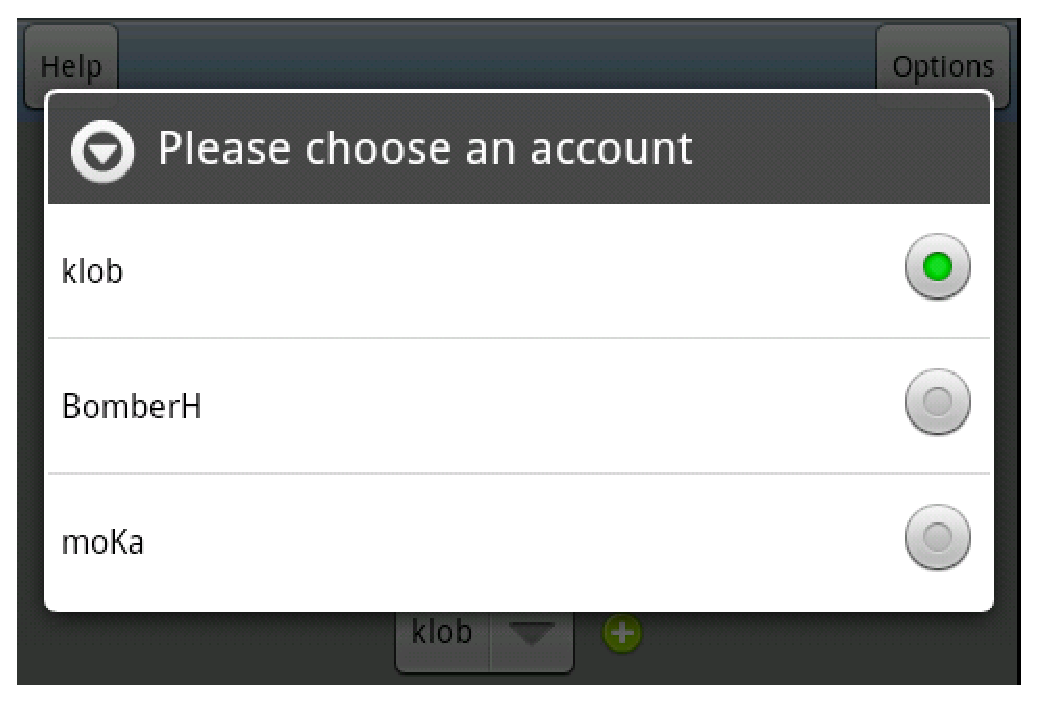
\includegraphics[scale=0.6]{Manuel/Img/8.eps}
	\end{center}
	
\newpage{}	

\paragraph{Ajouter compte local \textcolor{red}{6}\\}
	Il est nécessaire comme au premier lancement, de renseigner un pseudonyme 
	\textcolor{blue}{\textbf{1}}. Dans ce cas là une vérification de disponibilité
	de votre pseudonyme est faite. Une fois valide vous
	revenez sur le menu d'accueil avec votre nouveau compte local sélectionné.
	\begin{center}
		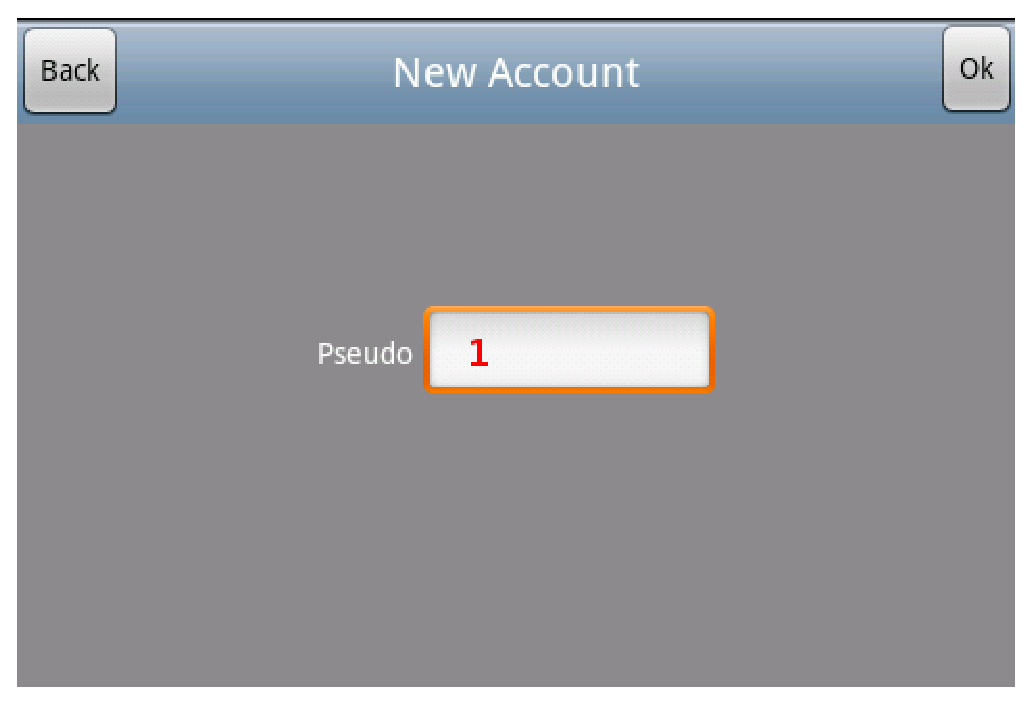
\includegraphics[scale=0.6]{Manuel/Img/9.eps}
	\end{center}
	
	
